\chapter{The Kalman Filter}
\label{ch:kf}

\begin{objectives}
\begin{itemize}
  \item Derive the Kalman filter from Bayes' rule and Gaussian conditioning, and recognize it as linear MMSE estimation and recursive
        least squares with dynamics.
  \item Understand the gain, the innovation and its covariance, the several equivalent forms of the covariance update, and the information form.
  \item Prove that the innovations of a correct filter are white, and use this to test filters without ground truth.
  \item Know why the Joseph form is used and how to implement the update without explicit inverses.
  \item Understand steady-state behavior, sequential updates, colored noise, continuous-time filtering and smoothing.
  \item Work a filter through by hand.
\end{itemize}
\end{objectives}

Rudolf Kálmán's 1960 paper~\cite{kalman1960} gave a recursive solution to linear estimation that needs only the current estimate and covariance.
It flew on Apollo and remains the backbone of navigation. This chapter derives it for linear systems; \cref{ch:nonlinear,ch:eskf} extend it to the
nonlinear, manifold-valued state of VIO.

% ==============================================================================
\section{The model}

A discrete-time linear system with Gaussian noise is described by (\cref{ch:linsys})
\begin{align}
  x_k &= \Phi_{k}\, x_{k-1} + w_k, & w_k &\sim \N(0, Q_k), \label{eq:lin-process}\\
  z_k &= H_k\, x_k + n_k, & n_k &\sim \N(0, R_k), \label{eq:lin-meas}
\end{align}
with $x_0 \sim \N(\hat x_0, P_0)$, and with $x_0$, $\{w_k\}$ and $\{n_k\}$ mutually independent and white. $\Phi_k$ is the state transition matrix, $Q_k$ the
process noise covariance, $H_k$ the measurement matrix and $R_k$ the measurement noise covariance; known inputs add a term $\Gamma_ku_k$ that only shifts
the mean. Continuous-time models are discretized as in \cref{sec:discretization}. The goal is the posterior $p(x_k \mid z_{1:k})$ given all
measurements up to time $k$.

% ==============================================================================
\section{The Bayes filter}

Two structural assumptions make recursion possible. The state is \emph{Markov}: given $x_{k-1}$, the earlier states and measurements carry no
further information about $x_k$. And each measurement depends only on the current state. Then the posterior can be computed recursively in two
steps:
\begin{align}
  \textbf{predict:}&\quad p(x_k \mid z_{1:k-1}) = \int p(x_k \mid x_{k-1})\, p(x_{k-1}\mid z_{1:k-1})\,\dd x_{k-1}, \\
  \textbf{update:}&\quad p(x_k \mid z_{1:k}) = \frac{p(z_k \mid x_k)\, p(x_k \mid z_{1:k-1})}{p(z_k\mid z_{1:k-1})}.
\end{align}
The prediction marginalizes the previous state out of the joint density $p(x_k, x_{k-1}\mid z_{1:k-1}) = p(x_k\mid x_{k-1})p(x_{k-1}\mid z_{1:k-1})$ (using the
Markov property); the update is Bayes' rule, with the new measurement independent of the past given the current state. For a linear-Gaussian
model all of these densities are Gaussian, so each step reduces to updating a mean and a covariance. We write $\hat x_k^-$, $P_k^-$ for the predicted
(prior) moments and $\hat x_k^+$, $P_k^+$ for the updated (posterior) moments.

% ==============================================================================
\section{Derivation}

\subsection{Prediction}

By \cref{prop:affine} applied to \eqref{eq:lin-process}, with $x_{k-1}$ and $w_k$ independent,
\begin{equation}
  \hat x_k^- = \Phi_k\,\hat x_{k-1}^+, \qquad P_k^- = \Phi_k P_{k-1}^+\Phi_k\T + Q_k .
  \label{eq:kf-predict}
\end{equation}
Prediction moves the error with the dynamics and adds process noise; it never decreases uncertainty in the directions excited by $Q_k$.

\subsection{Update}

Before the measurement arrives, the state and the measurement are jointly Gaussian. From \eqref{eq:lin-meas}, dropping the time index,
\begin{equation}
  \begin{bmatrix} x \\ z \end{bmatrix} \sim \N\!\left(
    \begin{bmatrix} \hat x^- \\ H\hat x^- \end{bmatrix},
    \begin{bmatrix} P^- & P^-H\T \\ HP^- & HP^-H\T + R \end{bmatrix} \right).
\end{equation}
Conditioning on the observed $z$ with \cref{thm:gauss-cond} gives the update directly.

\begin{theorem}[Kalman update]
\label{thm:kf-update}
\index{Kalman filter!update}\index{innovation}\index{Kalman gain}
Define the \term{innovation} (residual) $r = z - H\hat x^-$, its covariance $S = HP^-H\T + R$, and the \term{Kalman gain} $K = P^-H\T S\inv$. Then
\begin{equation}
  \hat x^+ = \hat x^- + K r, \qquad P^+ = P^- - K S K\T = (I - KH)\,P^- .
  \label{eq:kf-update}
\end{equation}
\end{theorem}
\begin{proof}
\Cref{eq:gauss-cond} with $\Sigma_{ab} = P^-H\T$ and $\Sigma_{bb} = S$ gives $\hat x^+ = \hat x^- + P^-H\T S\inv(z - H\hat x^-)$ and $P^+ = P^- - P^-H\T S\inv HP^-$. Since
$KSK\T = P^-H\T S\inv HP^- = KHP^-$, both covariance forms agree.
\end{proof}

The same formulas arise from the other routes of \cref{ch:estimation}: they are the linear MMSE estimate \eqref{eq:lmmse-update} (so the Kalman filter is the
best \emph{linear} filter even for non-Gaussian noise with the same second moments), the MAP estimate of \cref{prop:map-ls}, and recursive least squares
with a prediction step inserted between measurements.

\begin{keyidea}[the gain is a ratio of uncertainties]
For a scalar state measured directly ($H = 1$), $K = \frac{P^-}{P^- + R}$ and $P^+ = \frac{P^- R}{P^- + R}$. If the prior is much more uncertain than the
sensor ($P^- \gg R$), $K \to 1$ and the estimate jumps to the measurement. If the sensor is much worse ($R \gg P^-$), $K \to 0$ and the measurement is
nearly ignored. The posterior variance is always smaller than both. In general, $K$ maps the innovation, which lives in measurement space, into a
correction in state space, including corrections to states that are not measured directly but are correlated with measured ones through
$P^-$. This is how a pose measurement corrects velocity and biases.
\end{keyidea}

\subsection{The information form}

Applying the Woodbury identity (\cref{thm:woodbury}) to $P^+ = P^- - P^-H\T(HP^-H\T + R)\inv HP^-$ gives
\begin{equation}
  (P^+)\inv = (P^-)\inv + H\T R\inv H, \qquad K = P^+ H\T R\inv .
  \label{eq:kf-info}
\end{equation}
Information adds: each independent measurement contributes $H\T R\inv H$. The covariance form \eqref{eq:kf-update} inverts an $m\times m$ matrix ($m$ =
measurement dimension); the information form inverts an $n\times n$ matrix ($n$ = state dimension). Filters use the former when $m < n$; the
\emph{information filter}, which propagates $(P\inv, P\inv\hat x)$ instead, is preferred when measurements are many and large and the prediction step is
simple.

% ==============================================================================
\section{A worked example by hand}

\begin{worked}[a random walk observed directly]
A scalar state follows $x_k = x_{k-1} + w_k$ with $Q = 1$ and is measured as $z_k = x_k + n_k$ with $R = 2$. Start from $\hat x_0 = 0$, $P_0 = 4$, and receive
$z_1 = 1.5$, $z_2 = 2.0$.
\begin{center}\small
\begin{tabular}{@{}l l l@{}}
\toprule
 & $k = 1$ & $k = 2$ \\
\midrule
predict & $\hat x_1^- = 0$, $P_1^- = 4 + 1 = 5$ & $\hat x_2^- = 1.071$, $P_2^- = 1.429 + 1 = 2.429$ \\
innovation & $r_1 = 1.5$, $S_1 = 5 + 2 = 7$ & $r_2 = 2.0 - 1.071 = 0.929$, $S_2 = 4.429$ \\
gain & $K_1 = 5/7 = 0.714$ & $K_2 = 2.429/4.429 = 0.548$ \\
update & $\hat x_1^+ = 1.071$, $P_1^+ = 5\cdot2/7 = 1.429$ & $\hat x_2^+ = 1.071 + 0.548\cdot0.929 = 1.581$, $P_2^+ = 1.097$ \\
\bottomrule
\end{tabular}
\end{center}
The variance falls from 4 to about 1.1 in two steps and then settles where the information gained per measurement balances the uncertainty added per
step: solving $P^- = P^-R/(P^- + R) + Q$ gives $P^-_\infty = \tfrac12(Q + \sqrt{Q^2 + 4QR}) = 2$, $K_\infty = 0.5$, $P^+_\infty = 1$.
\end{worked}

% ==============================================================================
\section{Properties}

\begin{proposition}[Optimality]
For the linear-Gaussian model, $\hat x_k^+ = \E[x_k\mid z_{1:k}]$: the Kalman filter is the minimum mean-square error estimator among \emph{all} estimators,
linear or not (\cref{thm:mmse}). If the noises are not Gaussian but have the stated means and covariances, it remains the best \emph{linear}
estimator (\cref{thm:lmmse}).
\end{proposition}

\begin{proposition}[Innovation properties]
\label{prop:innovation}
If the model is correct, the innovations $r_k$ are zero-mean, Gaussian, with covariance $S_k$, and uncorrelated across time. Consequently
$r_k\T S_k\inv r_k \sim \chi^2_{m_k}$.
\end{proposition}
\begin{proof}
$r_k = H_k(x_k - \hat x_k^-) + n_k$ is a linear combination of zero-mean Gaussians; its two terms are independent, giving covariance
$H_kP_k^-H_k\T + R_k = S_k$. For whiteness, take $j < k$. The innovation $r_j$ is a linear function of $z_1, \dots, z_j$. The prediction error
$x_k - \hat x_k^-$ is uncorrelated with every past measurement by the orthogonality principle (\cref{thm:lmmse}), and $n_k$ is independent of the past;
hence $\E[r_kr_j\T] = H_k\E[(x_k - \hat x_k^-)r_j\T] + \E[n_kr_j\T] = 0$. The $\chi^2$ statement is \cref{thm:mahalanobis-chi2}.
\end{proof}

\Cref{prop:innovation} is the most useful diagnostic in filtering, because it can be checked on real data without ground truth. The \term{normalized
innovation squared} (NIS) $r\T S\inv r$ should look like a $\chi^2_m$ sample, and the innovation sequence should look white. Values that are
systematically too large mean the filter is overconfident or the model is wrong; systematically too small means it is underconfident;
correlation in time reveals unmodeled dynamics. Gating (\cref{ch:updates}) uses the same statistic one measurement at a time.

\subsection{Steady state}

For a time-invariant model, the covariance recursion does not depend on the measurements at all: it can be computed in advance. Substituting the
update into the prediction gives the \emph{discrete Riccati equation}
\begin{equation}
  P_{k+1}^- = \Phi\big(P_k^- - P_k^-H\T(HP_k^-H\T + R)\inv HP_k^-\big)\Phi\T + Q .
\end{equation}
If $(\Phi, H)$ is observable (more precisely, detectable) and $(\Phi, Q^{1/2})$ is controllable (stabilizable), $P_k^-$ converges to the unique positive
semi-definite solution of the algebraic Riccati equation obtained by setting $P_{k+1}^- = P_k^-$, from any initial $P_0$, and the gain converges to a constant.
The worked example shows this convergence. Navigation filters are not time-invariant, but the same balance between injected and gained
information governs them: in observable directions the covariance settles to a level set by the noise; in unobservable directions it does not
(\cref{sec:observability-linear}).

% ==============================================================================
\section{The Joseph form}
\label{sec:joseph}

\begin{proposition}[Joseph form]
\label{prop:joseph}
\index{Joseph form}
For \emph{any} gain $K$ (optimal or not), the error covariance after the update $\hat x^+ = \hat x^- + K(z - H\hat x^-)$ is
\begin{equation}
  P^+ = (I - KH)\,P^-\,(I - KH)\T + K R K\T .
  \label{eq:joseph}
\end{equation}
For the optimal gain it equals $(I - KH)P^-$.
\end{proposition}
\begin{proof}
The posterior error is $e^+ = x - \hat x^+ = (I - KH)(x - \hat x^-) - Kn$. Its two terms are independent, so by \cref{prop:affine} its covariance is
\eqref{eq:joseph}. Expanding with $K = P^-H\T S\inv$:
$(I-KH)P^-(I-KH)\T + KRK\T = (I-KH)P^- - (I-KH)P^-H\T K\T + KRK\T = (I-KH)P^- - P^-H\T K\T + K S K\T$, and the last two terms cancel because
$KSK\T = P^-H\T K\T$.
\end{proof}

Why use the longer formula? In floating point, $(I - KH)P^-$ is the difference of two nearly equal matrices when the update is informative, and it is not
symmetric. Rounding can push small eigenvalues negative, after which the filter is broken: variances become negative, Cholesky fails, gates
misbehave. The Joseph form is a sum of a congruence of $P^-$ and a congruence of $R$, so by \cref{prop:psd} it is PSD whenever $P^-$ and $R$ are,
regardless of rounding in $K$. It also remains correct when $K$ is deliberately suboptimal (for example, a gain computed with a slightly stale $P$).
AGENTS.md F3 mandates it.

\begin{implnote}[cost of the Joseph form]
With $n$ states and $m$ measurements, $(I - KH)P(I-KH)\T$ costs $\mathcal{O}(n^3)$ if done naively. For the MSCKF ($n = 75$) this is fine. If it ever
matters, note that the update can be rearranged as $P^+ = P - KHP - (KHP)\T + K S K\T$, which costs $\mathcal{O}(n^2 m)$ and is algebraically identical to the
Joseph form for any gain. It no longer has the sum-of-congruences structure that guarantees positive semi-definiteness under rounding, though, so
keep the symmetrization and monitor the smallest eigenvalue in tests. Profile before optimizing.
\end{implnote}

% ==============================================================================
\section{Implementing the update}

\begin{algorithm}[t]
\caption{Numerically careful Kalman update}
\label{alg:kf-update}
\begin{algorithmic}[1]
\Require prior $(\hat x, P)$, measurement $z$, model $(H, R)$
\State $r \gets z - H\hat x$ \Comment{innovation}
\State $S \gets HPH\T + R$; \quad $S \gets \tfrac12(S + S\T)$
\State $L \gets \mathrm{chol}(S)$ \Comment{or LDL$^\mathsf{T}$; failure means $S$ is not PD}
\State $\gamma \gets \|L\inv r\|^2$ \Comment{NIS, for gating and logging}
\If{$\gamma > \chi^2_{0.95}(\dim r)$} \State \Return reject (and count it) \EndIf
\State solve $S\,K\T = HP$ for $K\T$ using $L$ \Comment{never form $S\inv$}
\State $\hat x \gets \hat x + Kr$
\State $P \gets (I - KH)P(I - KH)\T + KRK\T$; \quad $P \gets \tfrac12(P + P\T)$
\end{algorithmic}
\end{algorithm}

\Cref{alg:kf-update} collects the numerical rules of the previous sections. Two details deserve comment. The gain is obtained by solving
$SK\T = HP\T = HP$ (since $P$ is symmetric), so the Cholesky factor of $S$ is reused for both the gate and the gain. And symmetrization after each step
removes the asymmetry that rounding introduces, which otherwise slowly accumulates (AGENTS.md F2).

\subsection{Sequential updates}

\begin{proposition}[Sequential processing]
If a stacked measurement $z = (z_1, z_2)$ has block-diagonal noise covariance $R = \blkdiag(R_1, R_2)$, updating with $z_1$ and then with $z_2$ gives
exactly the same posterior as a single update with $z$.
\end{proposition}
\begin{proof}
With independent noise blocks, the likelihood factorizes, $p(z\mid x) = p(z_1\mid x)p(z_2\mid x)$, so
$p(x\mid z) \propto p(z_2\mid x)\,\big[p(z_1\mid x)p(x)\big] \propto p(z_2\mid x)\,p(x\mid z_1)$: updating with $z_2$ the posterior after $z_1$. Both updates are exact for linear-Gaussian
models. (In information form: the information contributions $H_1\T R_1\inv H_1 + H_2\T R_2\inv H_2$ simply add.)
\end{proof}

Sequential processing can reduce cost (several small inversions instead of one large one) and allows per-block gating. If the blocks share errors
(correlated $R$), sequential processing without accounting for the correlation is wrong. For nonlinear models the two orders differ slightly,
because the second update is linearized at the estimate produced by the first.

% ==============================================================================
\section{Extensions}

\paragraph{Colored noise.} The derivation assumed white process and measurement noise. Time-correlated disturbances are handled by adding the state of
a shaping filter to the filter state (\cref{ch:processes}): this is why IMU biases, which are random walks, are state variables.

\paragraph{Continuous time: the Kalman--Bucy filter.} For continuous measurements $z(t) = Hx + n$ with white $n$ of density $R_c$, the limit of the discrete
filter as the sampling period goes to zero is
\begin{equation}
  \dot{\hat x} = F\hat x + K\big(z - H\hat x\big), \qquad K = PH\T R_c\inv, \qquad \dot P = FP + PF\T + GQ_cG\T - PH\T R_c\inv HP,
\end{equation}
a Lyapunov equation (\cref{prop:lyapunov}) with an information term subtracted. Navigation filters process sampled measurements and use the discrete
form, but the continuous form gives insight into steady-state behavior.

\paragraph{Smoothing.} A filter estimates $x_k$ from measurements up to time $k$. A \emph{smoother} also uses later measurements, which can only improve the
estimate. The Rauch--Tung--Striebel smoother runs a Kalman filter forward, storing $\hat x_k^\pm$ and $P_k^\pm$, and then sweeps backward:
\begin{equation}
  C_k = P_k^+\Phi_{k+1}\T(P_{k+1}^-)\inv, \qquad \hat x_{k|N} = \hat x_k^+ + C_k(\hat x_{k+1|N} - \hat x_{k+1}^-), \qquad P_{k|N} = P_k^+ + C_k(P_{k+1|N} - P_{k+1}^-)C_k\T .
\end{equation}
Real-time VIO is a filtering problem, but the MSCKF smooths in a limited sense: the past poses kept as clones in its sliding window are corrected by
every later update that involves them.

% ==============================================================================
\section{A simulated example}

\begin{figure}[t]
  \centering
  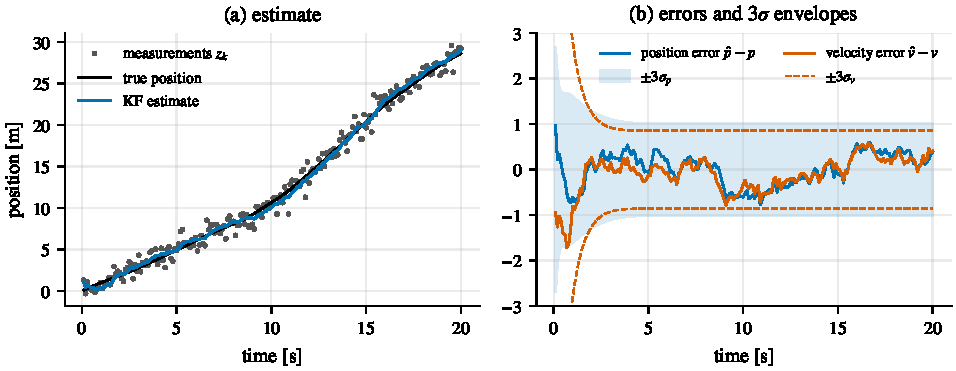
\includegraphics[width=\textwidth]{fig_kf1d.pdf}
  \caption{A constant-velocity Kalman filter tracking a 1D target from noisy position measurements. (a) The estimate smooths the measurements.
  (b) The errors stay inside the $\pm3\sigma$ envelopes, which shrink quickly from the uninformative prior and settle at the steady-state values set by
  the balance between process noise and measurement noise. The velocity is never measured, yet it is estimated through its correlation with
  position.}
  \label{fig:kf1d}
\end{figure}

\Cref{fig:kf1d} shows the filter on the constant-velocity model (\cref{ex:double-integrator-qd}), with position measurements at 10~Hz. Three behaviors
generalize to VIO. The covariance converges from its initial value to a steady state determined only by $Q$, $R$ and the geometry, not by the
data. The unmeasured state (velocity) is estimated through the correlation that the dynamics build up between position and velocity. And the errors
stay inside the $3\sigma$ envelope about 99.7\% of the time, the visual signature of a consistent filter.

\begin{takeaways}
\begin{itemize}
  \item Predict: $\hat x \gets \Phi\hat x$, $P \gets \Phi P\Phi\T + Q$. Update: condition the joint Gaussian of state and measurement.
  \item $K = PH\T S\inv$ maps innovations into state corrections, including corrections to unmeasured but correlated states.
  \item The Kalman filter is the exact Bayesian filter for linear-Gaussian models and the best linear filter otherwise.
  \item Innovations of a correct filter are white with covariance $S$; their NIS is $\chi^2$. This is testable without ground truth.
  \item Time-invariant observable systems reach a steady state set by the balance of process and measurement noise.
  \item Use the Joseph form, solve rather than invert, and symmetrize. Independent measurement blocks may be processed sequentially.
\end{itemize}
\end{takeaways}

\begin{exercises}
  \item Derive \eqref{eq:kf-update} for a scalar state measured twice by independent sensors of variances $R_1$ and $R_2$, first sequentially, then as a
        stacked 2D measurement. Show that the results agree.
  \item Show that $P^+ \preceq P^-$ for the optimal gain. Is this still true for an arbitrary gain in the Joseph form?
  \item Construct a $2\times2$ example in which $(I - KH)P^-$ computed in single precision is not positive semi-definite while the Joseph form is.
  \item Continue the worked example for five more steps and verify that $P_k^-$ converges to 2.
  \item For the scalar random walk with process variance $q$ and measurement variance $r$, derive $P^-_\infty = \tfrac12(q + \sqrt{q^2 + 4qr})$ and the
        steady-state gain. What happens as $q/r \to 0$ and $q/r \to \infty$?
  \item Implement \cref{alg:kf-update} in Python, reproduce \cref{fig:kf1d}, and compute the fraction of time steps where the position error lies outside
        $\pm3\sigma$.
  \item Test the whiteness of the innovations of your filter by computing their sample autocorrelation. Then mis-tune $Q$ and repeat.
\end{exercises}
